\documentclass[xcolor=dvipsnames,table]{beamer}

\usepackage{latexsym}
\usepackage[utf8]{inputenc}
\usepackage[brazil]{babel}
\usepackage{amssymb}
\usepackage{amsmath}
\usepackage{stmaryrd}
\usepackage{fancybox}
\usepackage{datetime}
\usepackage[T1]{fontenc}
\usepackage{graphicx}
\usepackage{graphics}
\usepackage{url}
\usepackage{algorithmic}
\usepackage{algorithm}
\usepackage{acronym}
\usepackage{array}

\newtheorem{definicao}{Definio}
\newcommand{\tab}{\hspace*{2em}}

\mode<presentation>
{
  \definecolor{colortexto}{RGB}{0,0,0}
 
  \setbeamertemplate{background canvas}[vertical shading][ bottom=white!10,top=white!10]
  \setbeamercolor{normal text}{fg=colortexto} 

  \usetheme{Warsaw}
}

\title{União e Intersecção de Grafos} 

\author{
  Esdras Lins Bispo Jr. \\ \url{bispojr@ufg.br}
  } 
 \institute{
  Teoria de Grafos \\Bacharelado em Ciência da Computação}
\date{\textbf{06 de junho de 2016} }

\logo{
\includegraphics[width=1cm]{images/ufgJataiLogo.png}}

\begin{document}

	\begin{frame}
		\titlepage
	\end{frame}

	\AtBeginSection{
		\begin{frame}{Sumário}%[allowframebreaks]{Sumário}
    		\tableofcontents[currentsection]
    		%\tableofcontents[currentsection, hideothersubsections]
		\end{frame}
	}

	\begin{frame}{Plano de Aula}
		\tableofcontents
		%\tableofcontents[hideallsubsections]
	\end{frame}
	
	\section{Pensamento}
	\begin{frame}{Pensamento}
  		\begin{center}
    		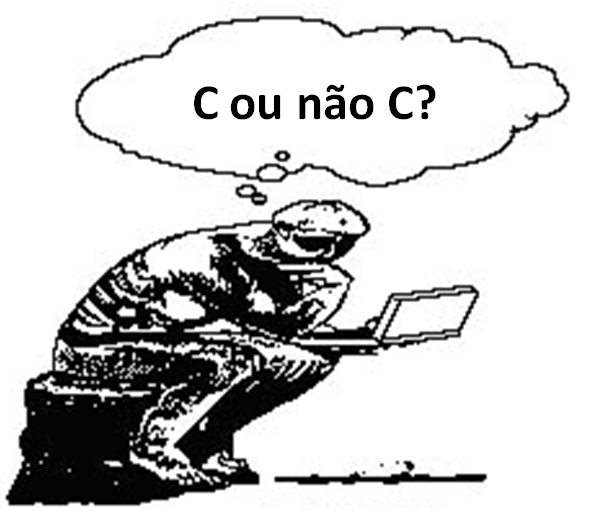
\includegraphics[width=7cm]{images/pensamento.png}
  		\end{center}
	\end{frame}
	
	\begin{frame}{Pensamento}
		\begin{columns}
			\column{.4\textwidth}  		
		  		\begin{center}
		    		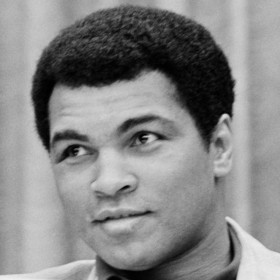
\includegraphics[height=.5\textheight]{images/ali.jpg}
		  		\end{center}
			\column{.6\textwidth}  		
				\begin{block}{Frase}
					\begin{center}
						{\large O impossível não é um fato, impossível é uma opinião.}
					\end{center}
				\end{block}		  		
		  		\begin{block}{Quem?}
		  			\begin{center}
						{\bf Muhammad Ali (1942-2016)} \\Pugilista e ativista estadunidense.
					\end{center}
				\end{block}
		\end{columns}
	\end{frame}
    
    \section{Revisão}
	\subsection{Grafos Conexos e Componentes}
	\begin{frame}{Grafos Conexos}
		\begin{block}{Definição}
			Um grafo é {\bf conexo} se, para qualquer par $\{v,w\}$ de seus vértices, existe um caminho com extremos $v$ e $w$.
		\end{block}
		\begin{block}{Subgrafo conexo maximal}
			Um subgrafo conexo $H$ de um grafo $G$ é maximal se $H$ não é subgrafo próprio de algum subgrafo conexo de $G$.
		\end{block}
		\begin{block}{Componente}
			Um {\bf componente} (ou {\bf componente conexo}) de um grafo $G$ é qualquer subgrafo conexo maximal de $G$.
		\end{block}
	\end{frame}
	
	\begin{frame}{Grafos Conexos}
		\begin{block}{Corolário 1}
			Cada vértice de um grafo pertence a um e um só componente.
		\end{block}
		\begin{block}{Corolário 2}
			 Um grafo é conexo se e somente se tem um único componente.
		\end{block}
	\end{frame}
	
	\section{União e Intersecção de Grafos}
	\begin{frame}{União e Intersecção de Grafos}
		\begin{block}{União}
			A {\bf união} de dois grafos $G$ e $H$ é o grafo $(V_G \cup V_H, E_G \cup E_H)$. É natural denotar esse grafo por $G \cup H$.
		\end{block} \pause
		\begin{block}{Intersecção}
			A {\bf intersecção} de dois grafos $G$ e $H$ é o grafo $(V_G \cap V_H, E_G \cap E_H)$. É natural denotar esse grafo por $G \cap H$.
		\end{block} \pause
		\begin{alertblock}{Alguns cuidados...}
			Para evitar grafos sem vértices, só trataremos da interação $G \cap H$ se $V_G \cap V_H$ não for vazio.
		\end{alertblock}
	\end{frame}
	
	\begin{frame}{União e Intersecção de Grafos}
		\begin{block}{Grafos disjuntos}
			Dois grafos $G$ e $H$ são {\bf disjuntos} se os conjuntos $V_G$ e $V_H$ são disjuntos.
		\end{block} \pause
		\begin{block}{Corolário}
		 	Se $G$ e $H$ são disjuntos, então $E_G$ e $E_H$ são disjuntos.
		\end{block}
	\end{frame}
	
	\begin{frame}{Bônus (0,5 pt)}
		\begin{block}{Desafio}
			\begin{itemize}
				\item {E 1.151} Prove que se um grafo $G$ é conexo, então seu complemento $\overline{G}$ é conexo; 
                \item Candidaturas até amanhã (07 de junho, 13h30); 
                \item Apresentação e resposta por escrito $\rightarrow$ \\segunda (14 de junho, 15h30); 
                \item 20 minutos de apresentação.
			\end{itemize}
		\end{block}
        \begin{block}{Referência}
			FEOFILOFF, P. {\bf Exercícios de Teoria dos Grafos}, \\
			BCC, IME-USP, 2012. 
		\end{block}	
	\end{frame}
	
	\begin{frame}
		\titlepage
	\end{frame}
	
\end{document}